\documentclass{article} % For LaTeX2e
\usepackage[dvipsnames]{xcolor}
% We will use NIPS submission format
\usepackage{nips13submit_e,times}
% for hyperlinks
\usepackage{hyperref}
\usepackage{url}
% For figures
\usepackage{graphicx}
\usepackage{subfigure}
\usepackage{caption}
%\usepackage{subcaption}
% math packages
\usepackage{amsmath}
\usepackage{amsfonts}
\usepackage{amsopn}
\usepackage{ifthen}
\usepackage{natbib}
% other
\usepackage{xspace}
\usepackage[]{algorithm2e}
\usepackage{paralist} % inline list
% e.g.:
% \begin{inparaenum}[a\upshape)]
% \item ...
% \item ...
% \end{inparaenum}

% Aliases
\newcommand{\TODO}[1]{\colorbox{YellowOrange}{\texttt{#1}}}

\title{Project-II by Group Ha-Noi}

\author{
Frederic Ouwehand \And Marco Antognini
}

\date{Fall 2015}

% The \author macro works with any number of authors. There are two commands
% used to separate the names and addresses of multiple authors: \And and \AND.
%
% Using \And between authors leaves it to \LaTeX{} to determine where to break
% the lines. Using \AND forces a linebreak at that point. So, if \LaTeX{}
% puts 3 of 4 authors names on the first line, and the last on the second
% line, try using \AND instead of \And before the third author name.

\nipsfinalcopy

\begin{document}

\maketitle

\begin{abstract}

This report states our findings and methodology for the image classification problem in Machine Learning using the Histogram of Oriented Gradients (HOG) and the \textit{Overfeat} Convolutional Network-based image features. We compare how the basic and the common advanced methods such as Support Vector Machines (SVM), Random Forests and Neural Networks compete in a binary and a multi classification task. We conclude with two prediction models and their respective expected error when classifying unseen images.

\end{abstract}

\section{Introduction}

The goal of this project is to predict whether an image contains a given object or not using machine learning techniques we have seen in class. For this particular real world problem, we focus on the identification of three kinds of objects: horses, planes and cars. If an image doesn't depict any of those categories, we consider it to belong to a fourth category "other". Moreover, we only consider images that contain exclusively one of the mentioned objects.

We focus on two separate but highly related tasks. On the one hand, we want to separate images that contain either a horse, a plane or a car from the ones that don't contain any of these objects. On the other hand, we are interested in classifying the images into the four above-mentioned groups.

In the remaining of this section we present the data on which our classification system is built upon as well as how we measure the expected error rate. We then quickly explain how we used a Principal Component Analysis (PCA) and why it was useful for our task. Next, we present the different methods used to classify images for the binary task and discuss their respective performance. Using these initial observations, we continue the discussion with the multi-class predictions and show how we can combine different classifiers to build more complex classification systems. In the following section we highlight a few implementation details and then report the result of our final classification systems. Finally, we summarise our findings and conclusions.

\subsection{Data Description}

To accomplish our goals we are given two set of features extracted from actual images for both training and testing data sets. For the training set we also have at our disposal the original 6,000 images from which the two sets of features were extracted in addition to the labels associated with the images. It is important to note that we don't have access to the original pixel representation of the images in the testing set and therefore we cannot extract additional features, say by applying contour detection or image skeletonisation, nor apply some unorthodox method, such as using well-known search engines to identify the source of the images.

The first set of features we have access to is histogram of oriented gradients (HOG), a feature descriptor based on oriented colour gradients and used initially to detect pedestrians in [\textit{HOG}]
%Navneet Dalal and Bill Triggs / http://ieeexplore.ieee.org/xpl/articleDetails.jsp?arnumber=1467360
and was later used for more diverse object detection in static images. For this project, it corresponds to a 5,408-dimensional feature vector per image sample that was generated using [\textit{PMT}] with 17 spacial bin and 8 orientation bins.

As shown in Figure \ref{fig:illustration-hog}, using this descriptor on images with few details can reveal the most important traits of the image but fails to produce a meaningful interpretation for more complex images, at least from the point of view of human beings.

\begin{figure}[h]
  \center
  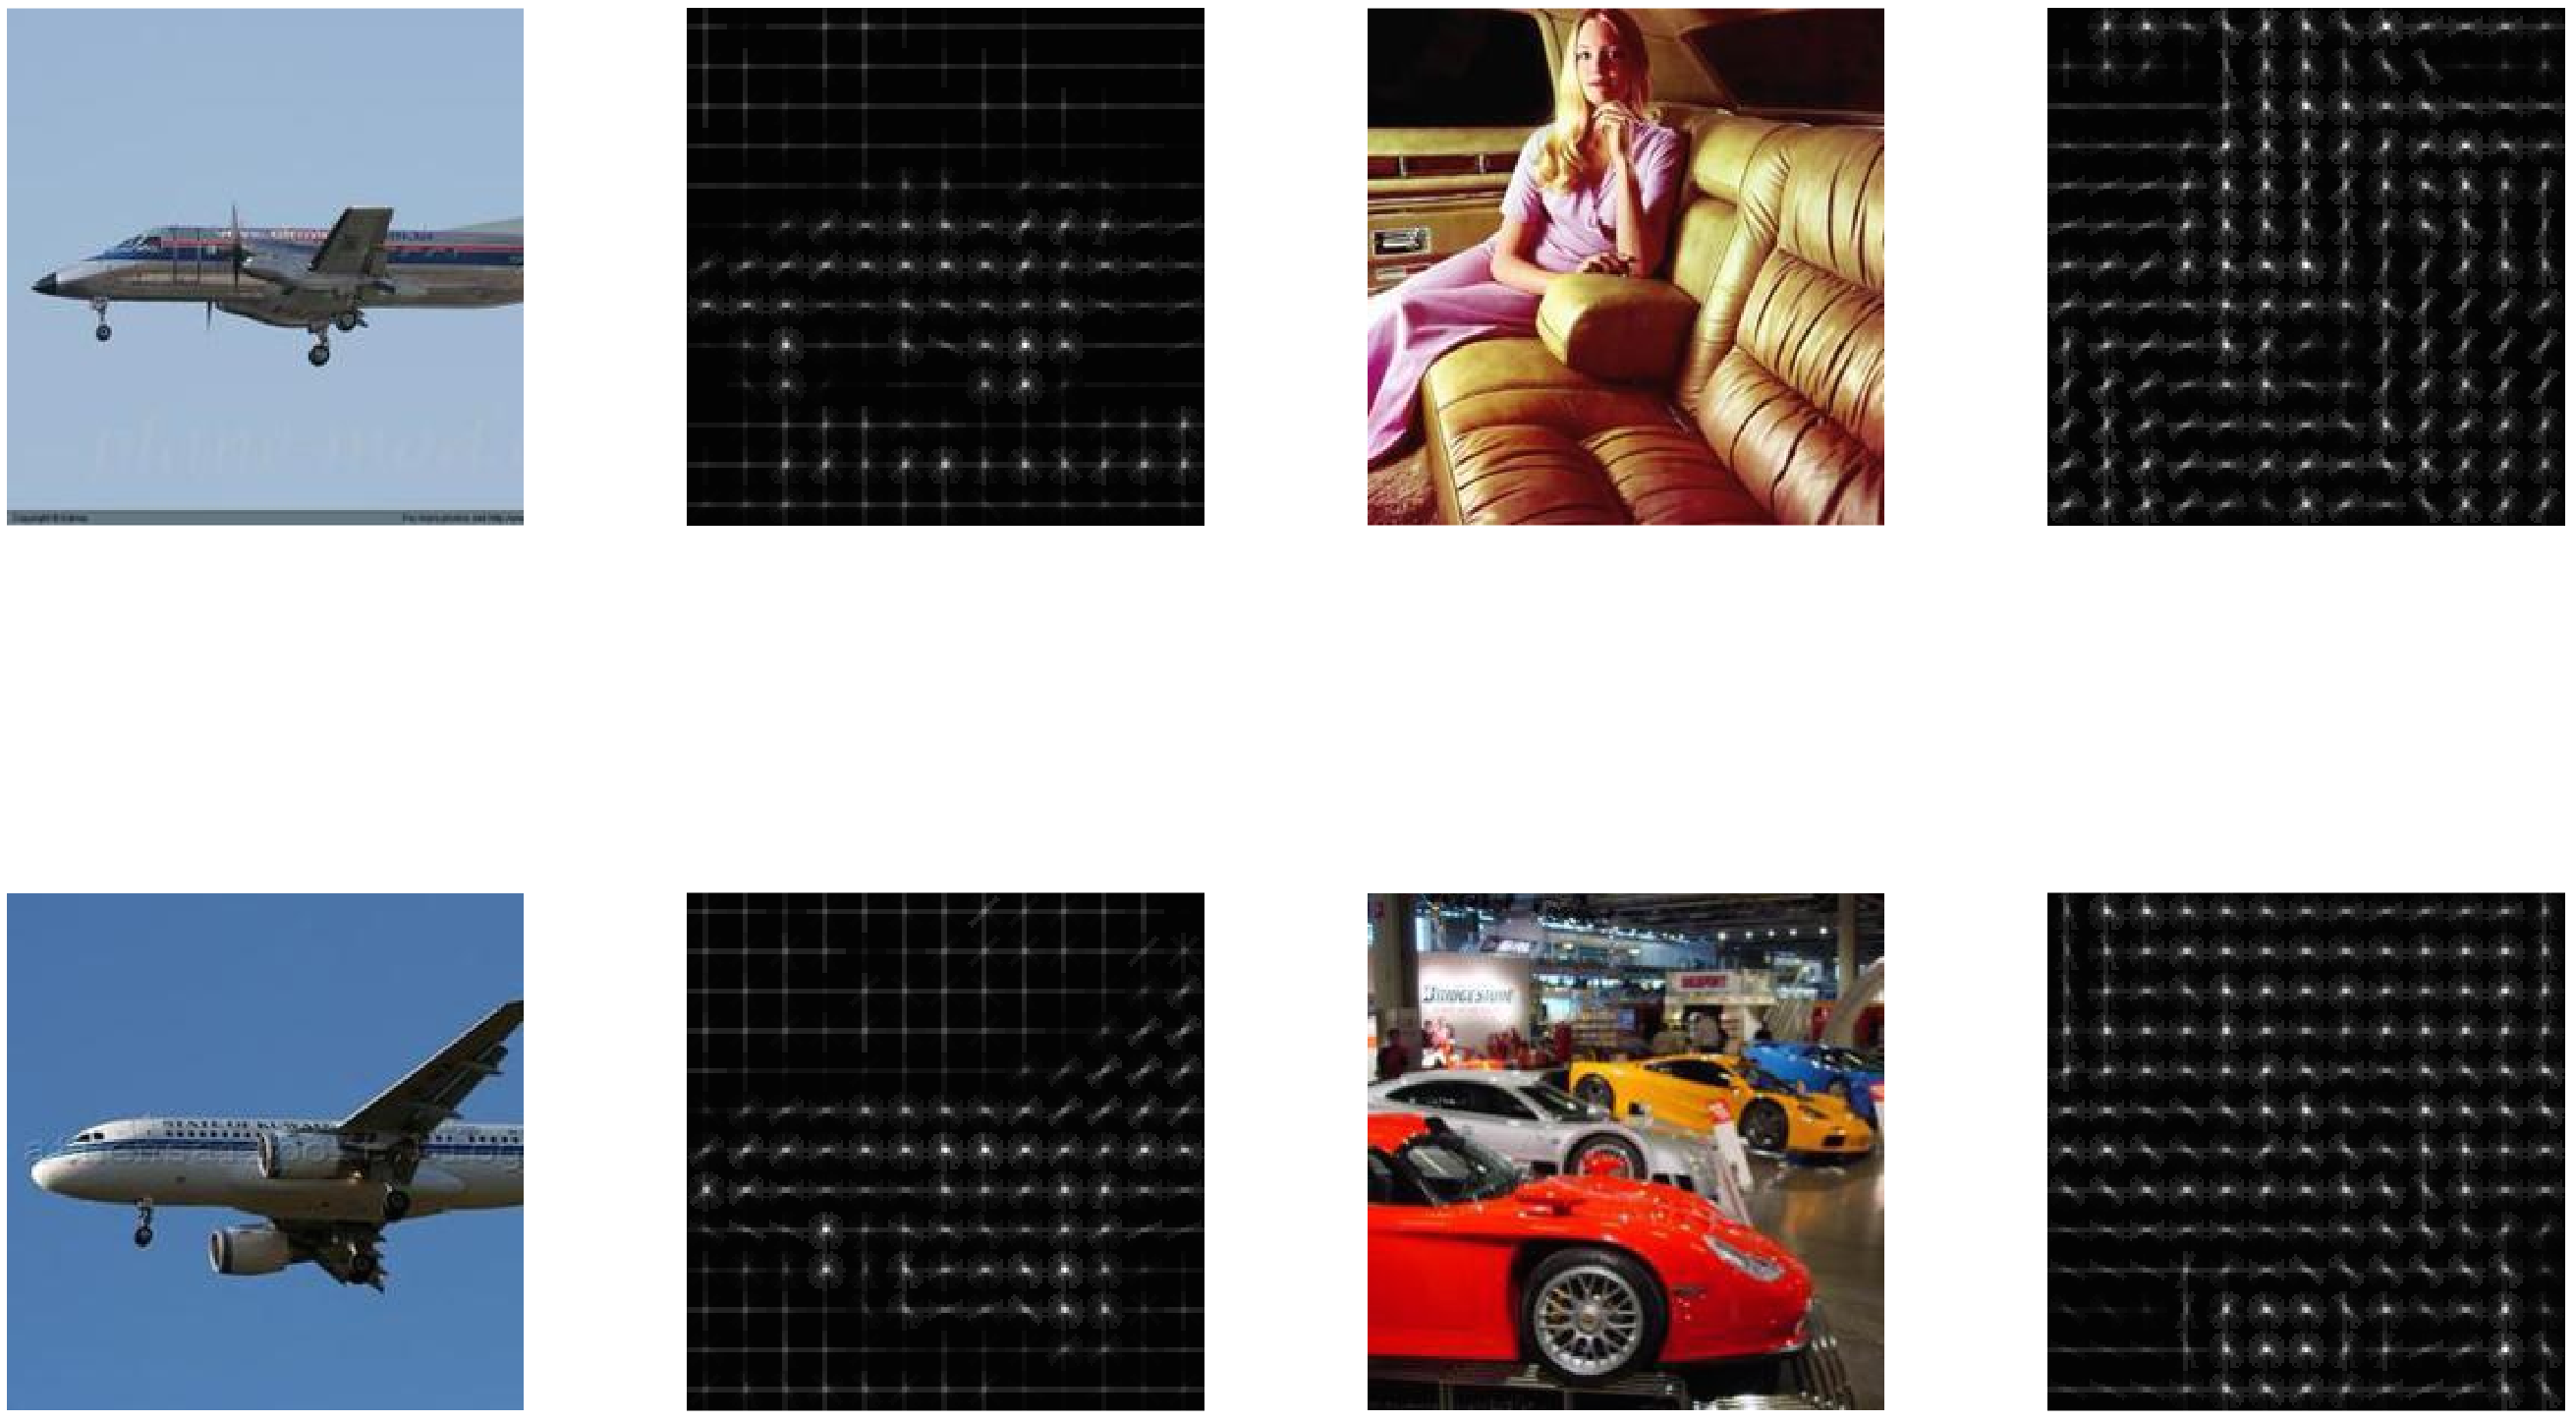
\includegraphics[width=0.7\textwidth]{figures/illustration_hog}
  \caption{Visualisation of HOG features for simple and complex images}
  \label{fig:illustration-hog}
\end{figure}

The second available feature set is based on the data extracted using OverFeat, a Convolutional Network-based image classifier and feature extractor that was trained on the ImageNet dataset as described in [\textit{OverFit}].
%OverFeat: Integrated Recognition, Localization and Detection using Convolutional Networks / http://arxiv.org/pdf/1312.6229.pdf or http://www.image-net.org/challenges/LSVRC/2013/slides/overfeat\_ilsvrc2013.pdf
For this feature set, we have for each of the 6,000 training images a very sparse representation of 36,865 data points and, unlike the previous set of features, cannot be trivially represented graphically.

Since the OverFeat features were generated using a Convolutional Neural Network we will refer to it as CNN in the remaining of the report.

Finally, the label distribution is reported in Figure \ref{fig:data-distribution}. As we can see, the training data is not equally distributed among classes: a large majority of the data belongs to the category "other".

While examining some of the misclassifications we noticed that a few images classified in the \textit{other} category were in fact horses, cars or planes. We identified about fifty misclassified images in the training set, which accounts for less than 1\% of the data and therefore should not significantly impact our predictions.

\begin{figure}[h]
  \center
  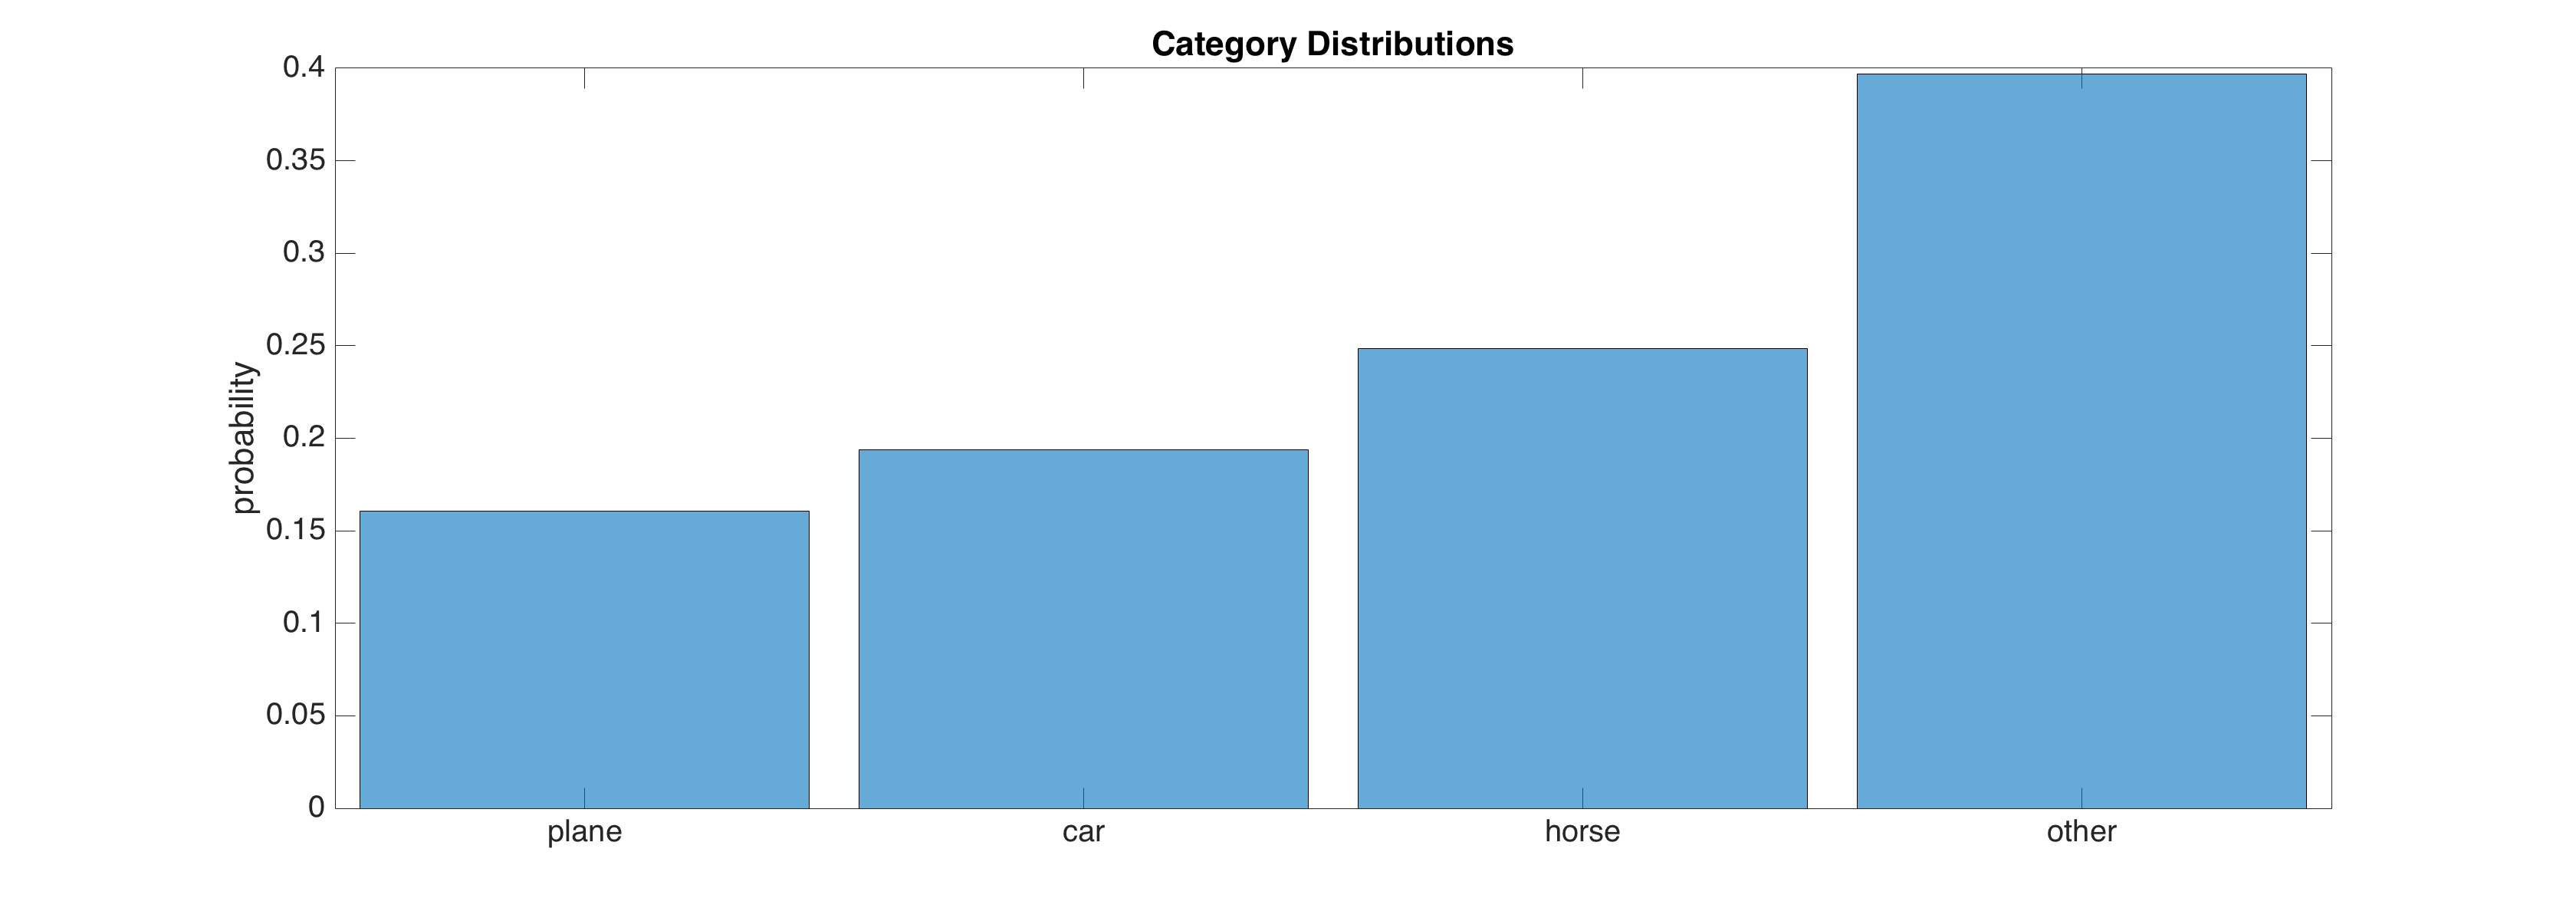
\includegraphics[width=\textwidth]{figures/data_distribution}
  \caption{Data distribution for the training data}
  \label{fig:data-distribution}
\end{figure}

\subsection{Error Metric}

While 0-1 loss can give some information about the accuracy of a system, this error metric doesn't take into account the distribution of the data among classification groups. If the distributions of the data for each class are equivalent then this is not an issue. However, as we have previously shown, our data is not well distributed among classes: e.g. the images of planes account only for 16\% of our training data. Hence, we need to measure our misclassification error more carefully in order to be resistant to the unbalanced nature of the data.

To solve this issue, we used the Balanced Error Rate (BER), whose formula is shown in Equation~(\ref{eq:BER}), that basically produces an average of the error per class and therefore reports a meaningful information even when 40\% of our training data represent images in the category "other". This means that if our predictor is utterly bad at categorizing cars then the resulting BER will be high, even if it is good at predicting horses and planes.

\begin{equation}
	\label{eq:BER}
    BER = \frac{1}{C}\sum_{c=1}^C \left[ \frac{1}{N_c} \sum_{n=1}^N \left(y_n = c\right) \left(y_n \neq \hat{y}_n \right) \right]
\end{equation}

In Equation~(\ref{eq:BER}), $C$ denotes the number of classes, $N_c$ is the number of examples in class $c$, $y_n$ represents the ground truth and $\hat{n}_n$ its corresponding prediction for sample $n$ out of $N$. For example, associating an image in a random binary or quaternary class will result in a BER close to 50\% and 75\%, respectively.

\subsection{Principal Component Analysis (PCA)}

Before thinking about applying any prediction model, we realised that the dimensionality of the provided features would be an issue. For HOG features, while still computationally possible, using the full set of features would result in a computational time blow-up with some methods such as Logistic Regression. As for the CNN features, naively using the full set of data would simply not be possible with regular computers, without mentioning theoretical issue due to the curse of dimensionality.

We therefore need a way to reduce the dimensionality of our data space. In order to select the right features from the data and leave out less relevant information, we decided to use Principal Component Analysis (PCA) to compress the data.

In order to tune the compression/loss ratio, we plotted the sum-of-squares distortion $J$ as introduced in Section 12.1 of [\textit{Bishop}].
We can infer from Figure \ref{fig:distortion-hog} that reducing the dimensionality to $M \approx 400$ for HOG features results in a distortion of less that 10\%. In practice, we have notice that reducing the dimensionality even further still yields good results.

\begin{figure}[h]
  \center
  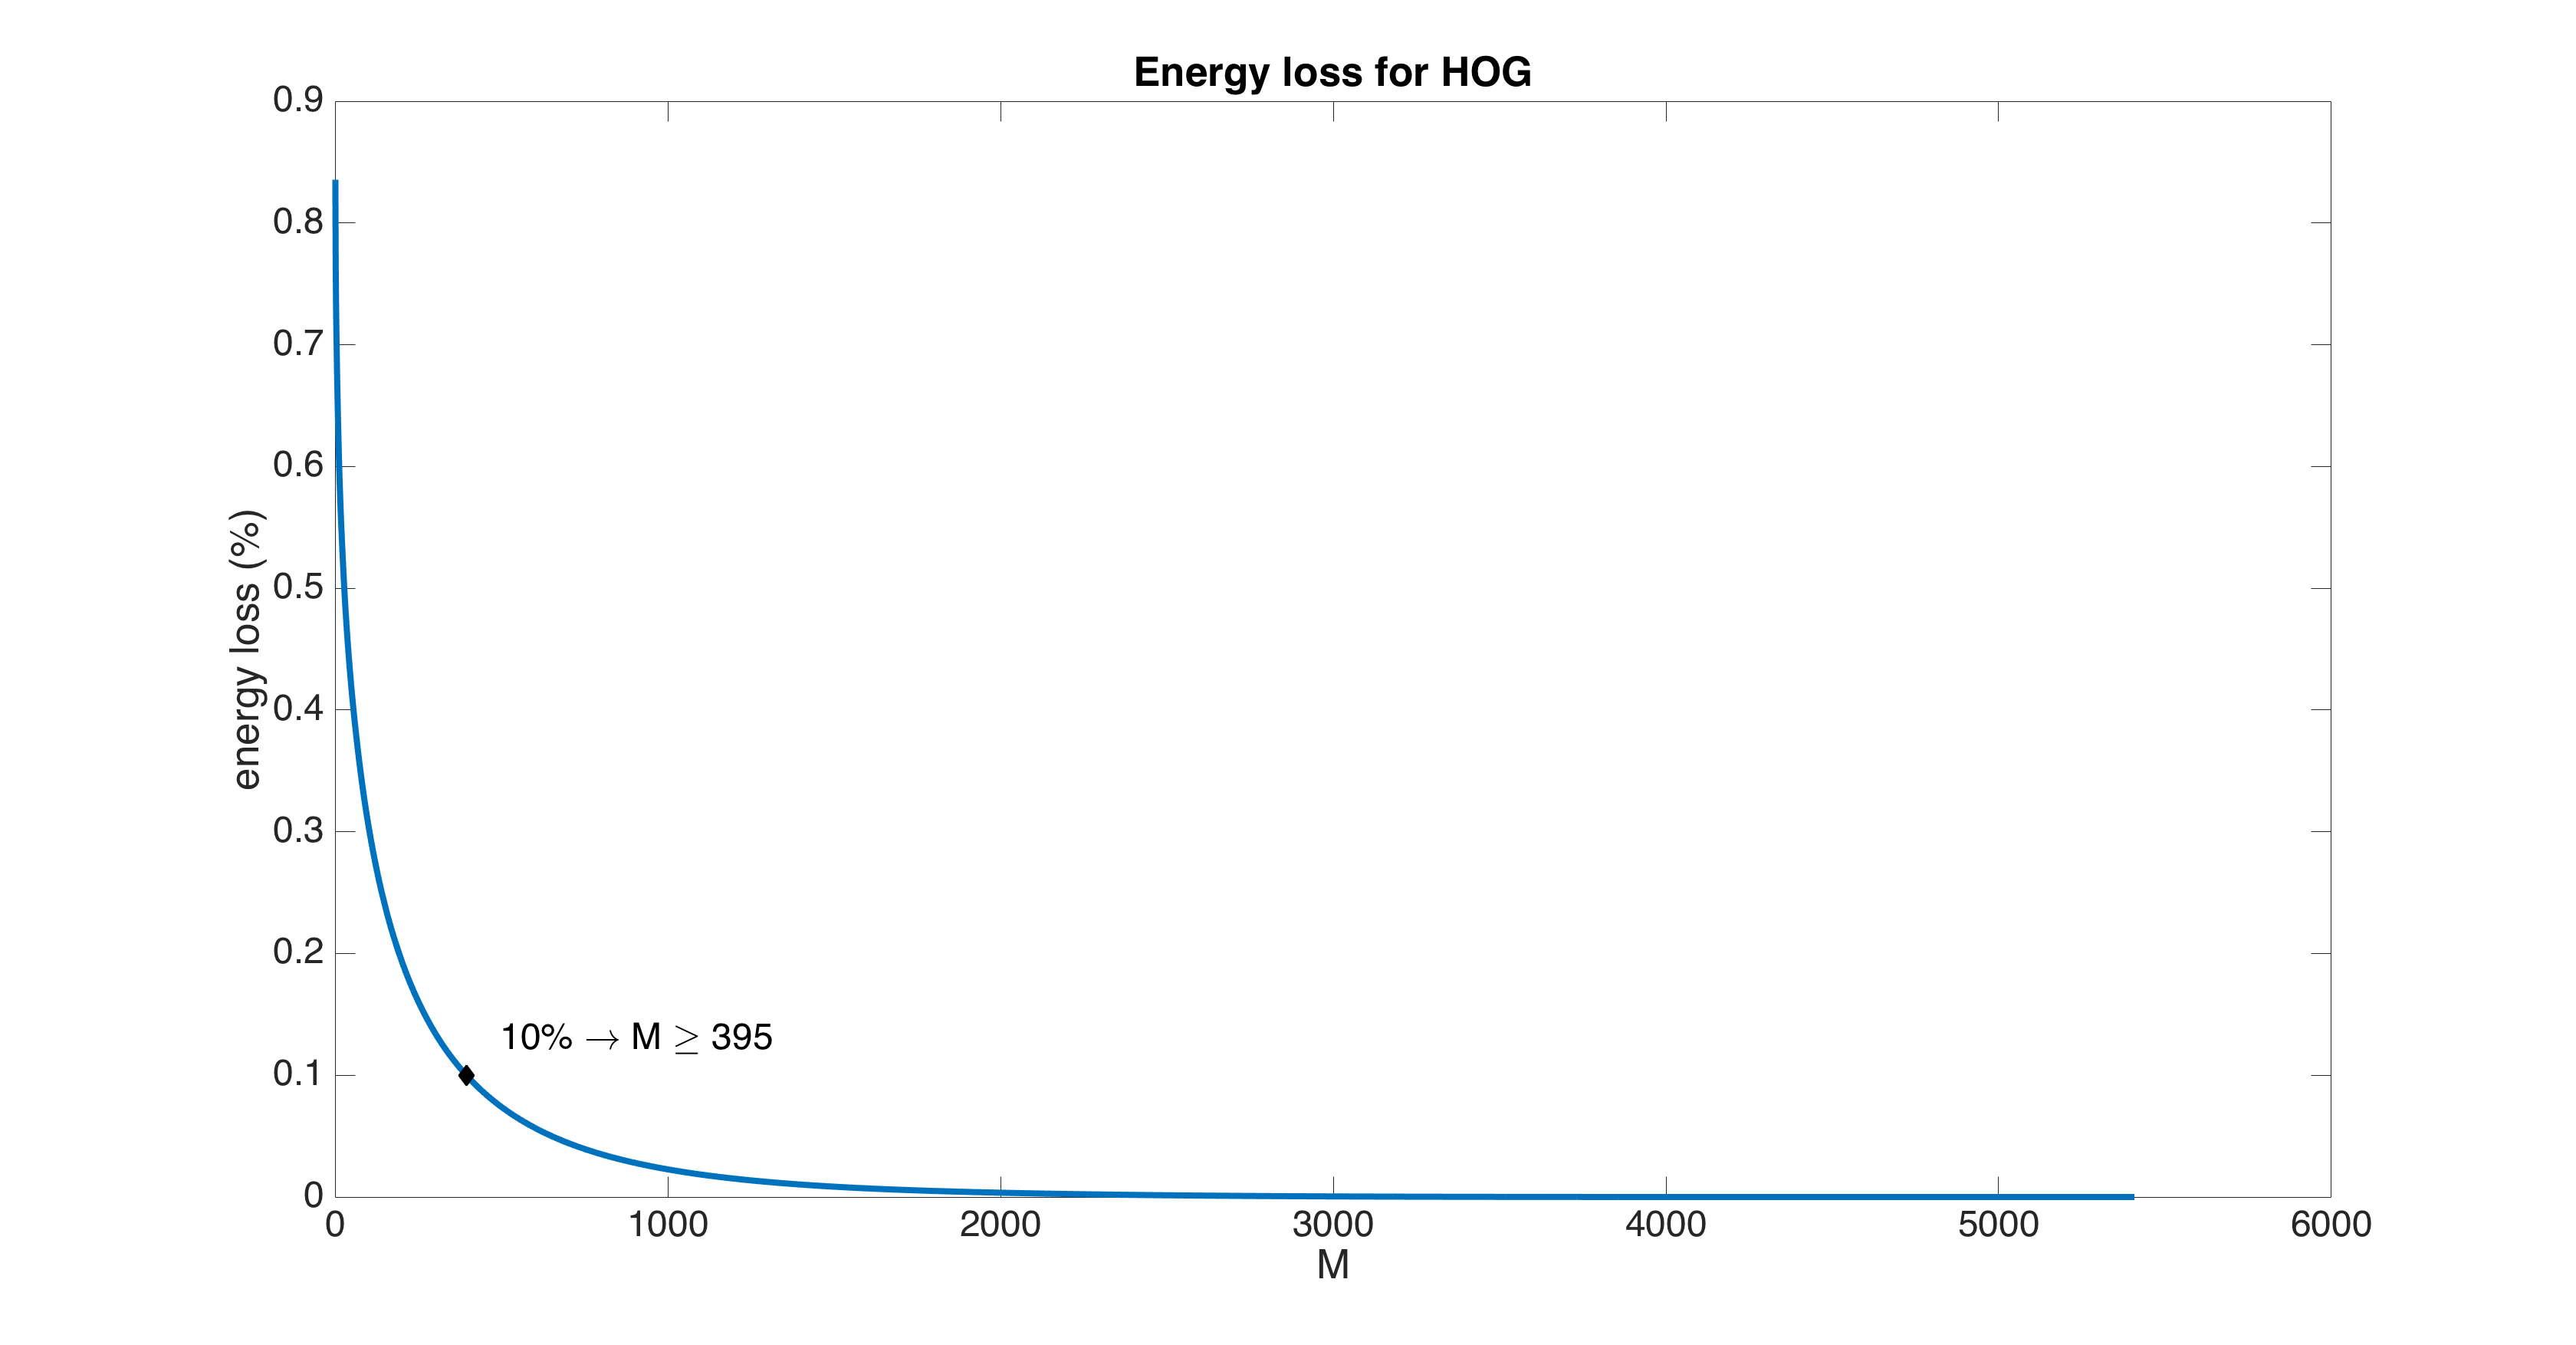
\includegraphics[width=\textwidth]{figures/distortion_energy_hog}
  \caption{Energy Loss of the HOG matrix}
  \label{fig:distortion-hog}
\end{figure}

As for CNN features, since its dimensionality exceeds the number of samples at our disposal, we have to use a trick in order to compute the eigenvectors as detailed in Section 12.1.4 of [\textit{Bishop}].
Beside the implementation issue for high-dimensional data, the curve shown in Figure \ref{fig:distortion-cnn} is pessimistic: since we only have 6,000 image samples, 30,865 of the 36,865 eigenvalues, that could exist were we to have 30,865 additional samples, are null. Therefore the distortion curve let us think that we need at least $M \approx 4000$ in order to retain 90\% of the information. However, in practice we have noted that using $M = 200$, or even smaller, could achieve good results.

\begin{figure}[h]
  \center
  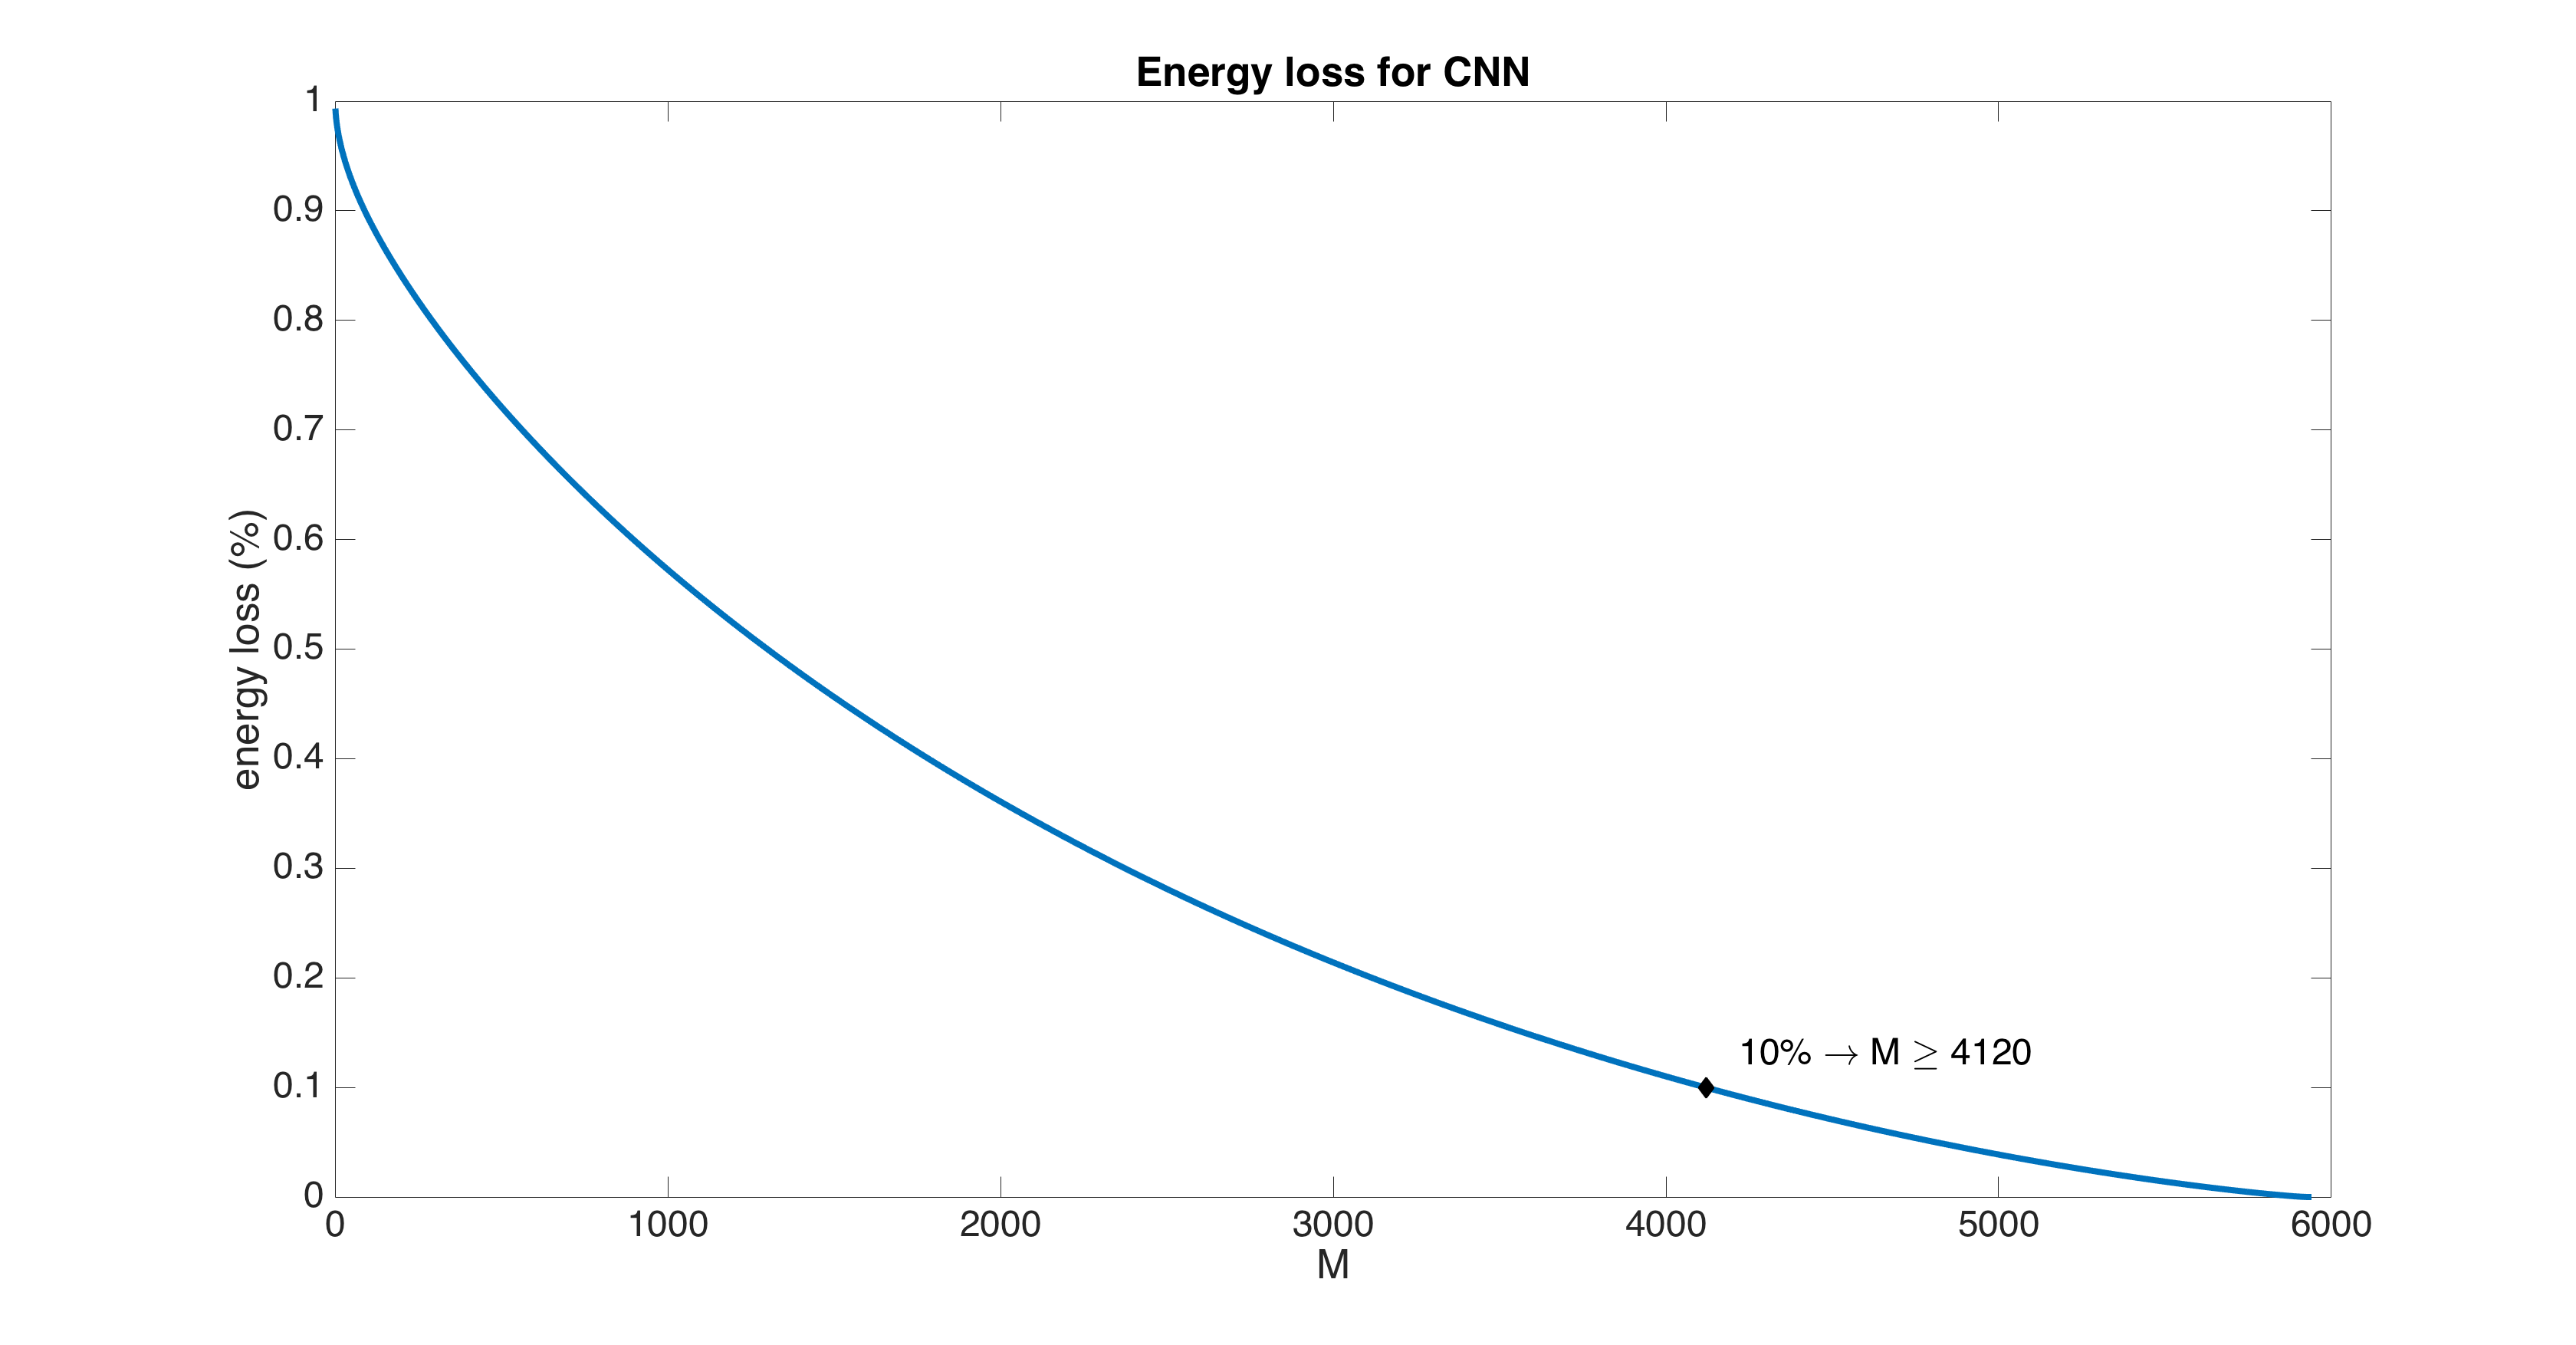
\includegraphics[width=\textwidth]{figures/distortion_energy_cnn}
  \caption{Energy Loss of the CNN matrix}
  \label{fig:distortion-cnn}
\end{figure}

\section{Binary classification}
\label{sec:binary}
Several methods were evaluated on the dataset using the training/validation methodology with a 0.7/0.3 ratio. The evaluation was repeated 20 times with a different random permutation of the images and produces an approximation of the Balanced Error Rate (BER) and a variance for each method. A full comparison is shown in Figure \ref{fig:methods-binary}, in which each method is shown with its error on the validation set. Note that methods use exclusively the training set to compute their models. Hence, hyper parameters such as C for SVM or gamma for the RBF kernel are computed using the training data which may be split into training/testing pieces in the case of K-Fold. The intuition is that our final error estimate should not be computed using data that has been used to tune our models.

\subsection{Path to the best model}

Logistic Regression is chosen as a baseline method for this classification task because of its simple and intuitive theoretical foundations. However, it relies on the optimization of the problem directly defined by the observations which is computationally expensive when the data samples have a high dimensionality such as the HOG and CNN features. The principal component algorithm was used to project the high frequency features on the principal axis found in our data in order to reduce the dimensionality of the HOG and CNN features to $15$ and $20$ respectively. These parameters were chosen after a 10-Fold cross-validation among other candidate values and were selected to minimize the expected error. We used the gradient descent method with line search to find an optimal solution. The penalized logistic regression method on the HOG and CNN features after applying the PCA algorithm is shown in the {$1$}st and the {$7$}th column of Figure \ref{fig:methods-binary} under the labels \textit{log reg HOG} and \textit{log reg CNN} and the BER is $28$\% and of $11$\% respectively. Polynomial features transformations $\Phi = \left[ x_{n}^{0.5}, x_{n}^2, x_{n}^3 \right]$ did not improve significantly the model.


\begin{figure}[h]
  \center
  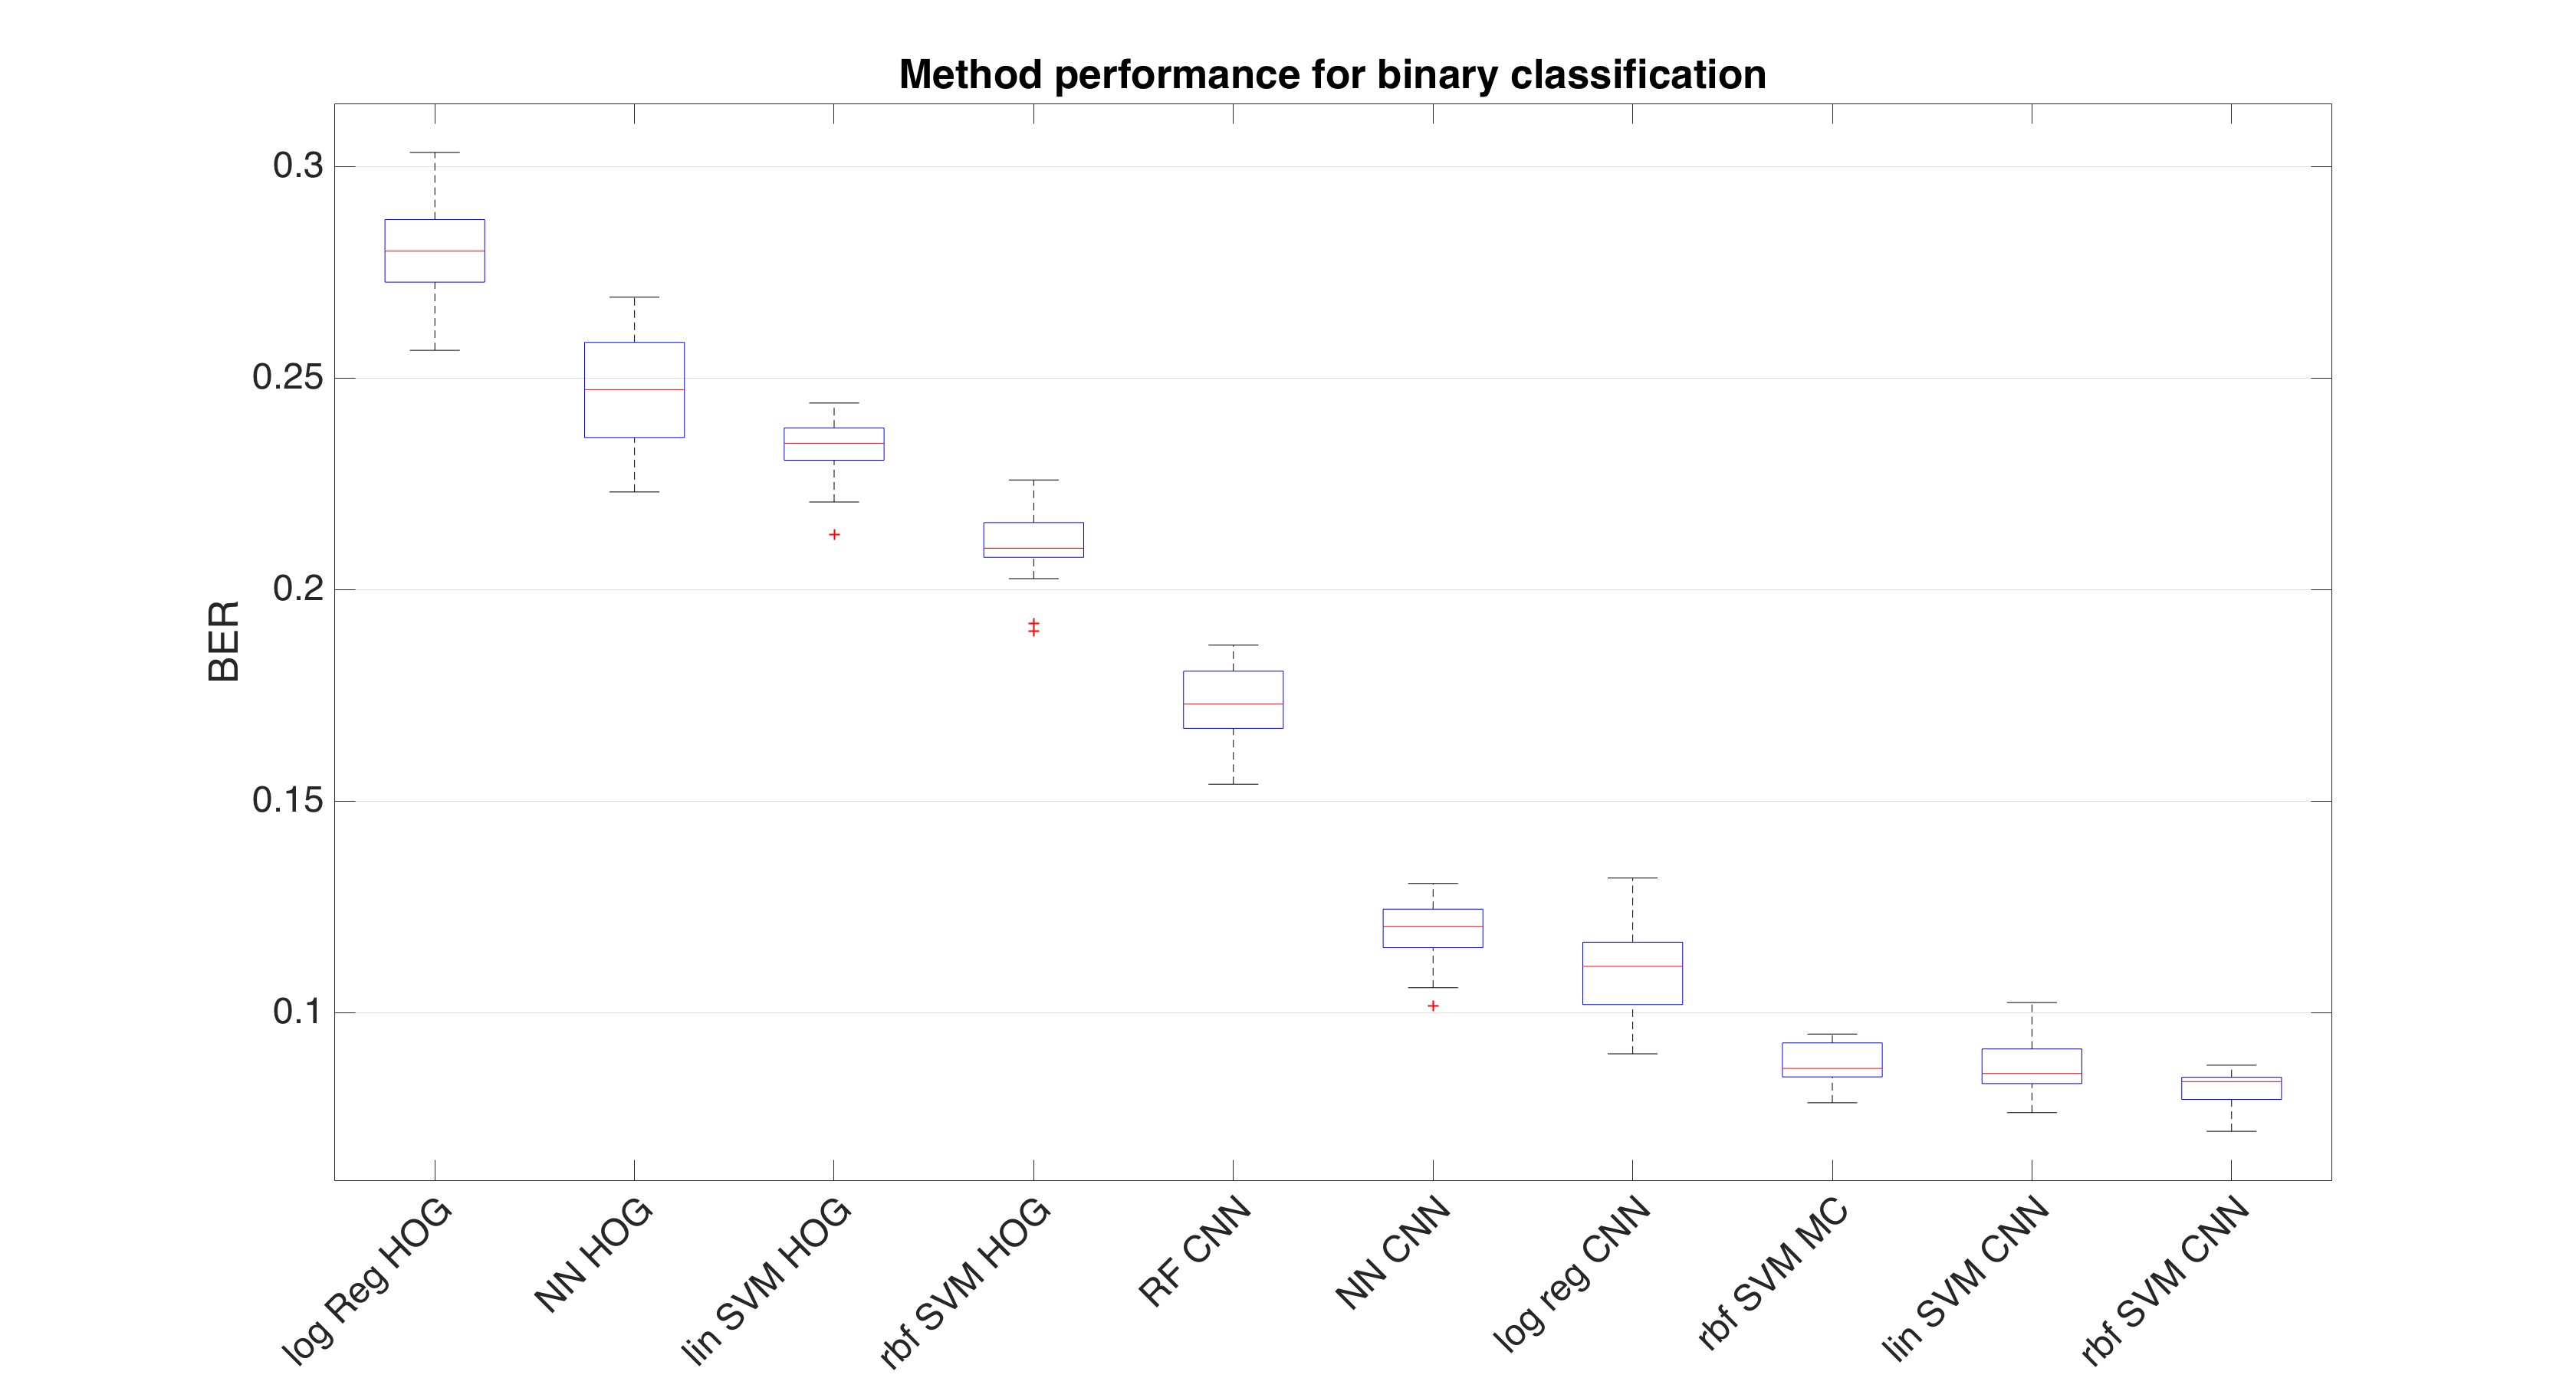
\includegraphics[width=\textwidth]{figures/binary_methods}
  \caption{Evaluating the methods for the Binary Task}
  \label{fig:methods-binary}
\end{figure}

Neural network are powerful since they can model any kind of function using internal neurons and many libraries propose fast implementations iteratively absorbing the data in small batches such as [\textit{DLT}]. The Neural Network method performed slightly better than the logistic regression on the HOG feature but worse on the CNN feature with respectively $25$\% and $12$\%. Overfitting was prevented by setting a low number of internal nodes in our network but few tuning was done on the model parameters since we realized that the Neural networks are extremely sensitive to their initialization which makes them hard to tune finely.

We preferred to investigate more stable models such as the Support Vector Machine model which does have the computational advantage of working on the dual problem since the number of HOG and CNN features is equivalent for HOG and six times bigger for CNN than the number of data samples. After training our model, the kernel for the prediction task is computed using the few training points associated with the support vectors and a final confidence score is produced for each unseen data point. Values between $-1$ and $1$ correspond to points that lie inside the margin in one or the other side of it and the absolute values bigger than $1$ are points for which the method is more confident about. Figure \ref{fig:missclassification-vs-svm-score} shows that very few images are misclassified by SVM when their score is above or below $1$.
Compared to the Neural Network, the Linear kernel offers a $5$\% and $28$\% improvement for the HOG and CNN features respectively with a low variance in both cases. To reduce the computational load, the PCA algorithm is applied to CNN before SVM. We chose to select only the first $150$ principal components from the CNN features matrix since the SVM algorithm performs equivalently well than with more principal components in this specific case.

The Polynomial kernels with degree $2$ and $3$ give slightly better classifications but the Radial Basis Function (RBF) clearly outperforms the Linear kernel by a $10$\% and a $2$\% reduction of the BER when applied on  the HOG and CNN features respectively. We used the Gaussian type of RBF Kernel defined by $k\left(x,x'\right)=e^{-\gamma\left\Vert x-x'\right\Vert ^{2}}$ where $\gamma$ is inversely proportional to the variance of the Gaussian distribution $\gamma\approx$$\frac{1}{2\sigma^{2}}$. We had to take a very big $\sigma$ since the high dimensionality of the data points make them appear to be very far from each other.

Anticipating the next multiclass predictions, Figure \ref{fig:cross-validation-rbf-hog} shows that $\gamma=1.9^{-3}$ and $C=9$ are the best parameters for the RBF SVM model applied on the HOG feature for predicting the car label versus the other labels. Similar cross validation on the hyper-parameters were computed for finding the optimal parameters of the Support Vector Machine algorithm for the other classes. The SVM method with a RBF kernel is shown in Figure \ref{fig:methods-binary} in column $4$ and $10$ under the labels \textit{rbf svm hog} and \textit{rbf svm cnn}, respectively.

Random Forests is an efficient method which can be applied on the CNN feature without any preprocessing. It is shown under the label \textit{RF (Random Forest) CNN} and achieves a BER score of $17.3$\% by averaging the predictions of $180$ trees with a maximal depth of $7$.

Our best and final model for the binary classification task is SVM with the RBF kernel on the CNN feature with $\gamma=2.3^{-4}$ and $C=3.25$ after applying the PCA algorithm on the $150$ biggest singular values. This method has a median BER score of $8.38$\% with a $0.52$\% difference between the $75$th and the $25$th quantile and a mean of $8.18$\%.

One could argue that the information lying in the HOG and CNN features may be combined to build a better model. However, decision trees or advanced methods such as Adaboost were not useful in combining our HOG and CNN models since their error rates highly differ. Models using the HOG feature range from a BER of $28$\% to a BER of $21$\% and the models based on the CNN feature score between $17$\% and $8.37$\%. However, we know from Figure \ref{fig:missclassification-vs-svm-score} that the error rate of the SVM models is inversely proportional to the absolute value of their output. Based on this observation, we tried to combine the SVM models and to make them vote by taking the prediction of the SVM method which outputs the maximum absolute value for a given data point. Figure \ref{fig:methods-binary} shows  this combination method in the $8$th column under the label \textit{rbf svm MC (Maximum Confidence)} with a BER of $8.7$\% which is greater than the RBF SVM on the CNN features.

\begin{figure}
  \center
  \subfigure[Correlation between the SVM score and the misclassification rate]{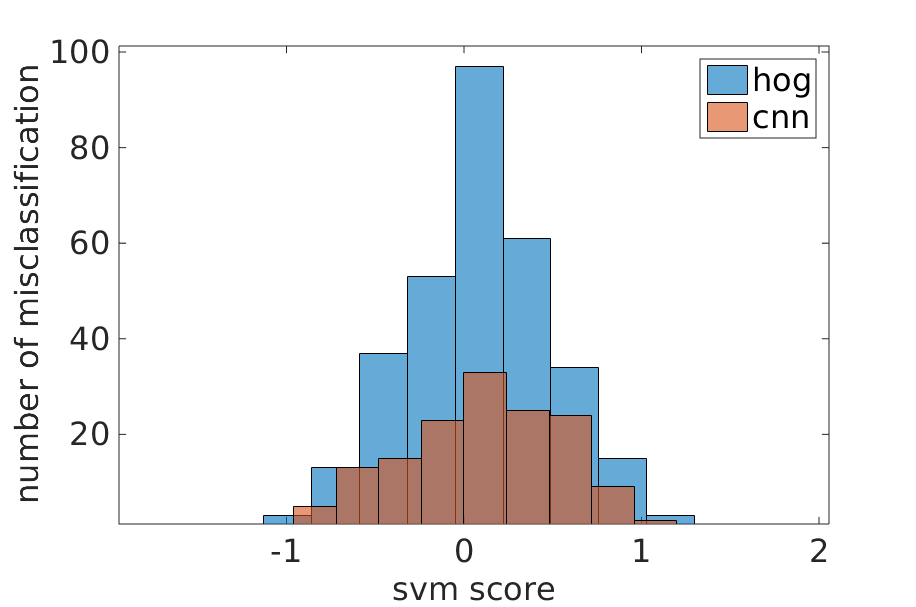
\includegraphics[width=0.48\textwidth]{figures/misclassification-vs-svm-score} \label{fig:missclassification-vs-svm-score}}
  \hfill
  \subfigure[Cross-validating the gamma and C parameters for SVM with RBF kernel on hog for the classification car vs other]{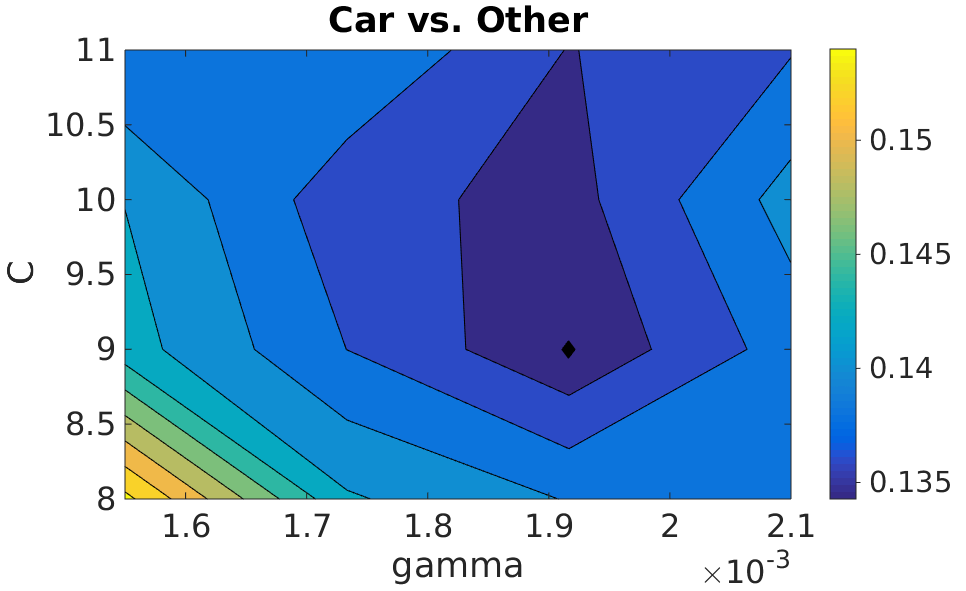
\includegraphics[width=0.48\textwidth]{figures/cross-validation-rbf-hog} \label{fig:cross-validation-rbf-hog}}
  \caption{Validation BER for each method of the binary classification}
  \label{fig:lambdas}
\end{figure}

\section{Multi-class classification}

Based on our previous findings, we decided to solve the multi-class problem by testing three main strategies. First, we applied the best known method for binary classification to independently identify images from the \textit{car}, \textit{horse} and \textit{plane} categories to generate three confidence scores. As Figure \ref{fig:svm-binaries} shows, using our previously build SVM model with RBF kernel, we were able, after carefully tuning the different parameters of the models, to detect whether a car is present in an image with an accuracy superior to 97\%; detecting planes or horses is slightly harder with an accuracy of 95\% and 93\%, respectively and finally the accuracy of identifying images from the category \textit{other} is down to 91\%. Those results were obtained by using the CNN features. However, when we used the HOG features instead we achieved an accuracy several magnitude lower but with similar relative performance which means that cars are consistently simpler to identify with both set of features.

\begin{figure}[h]
	\center
	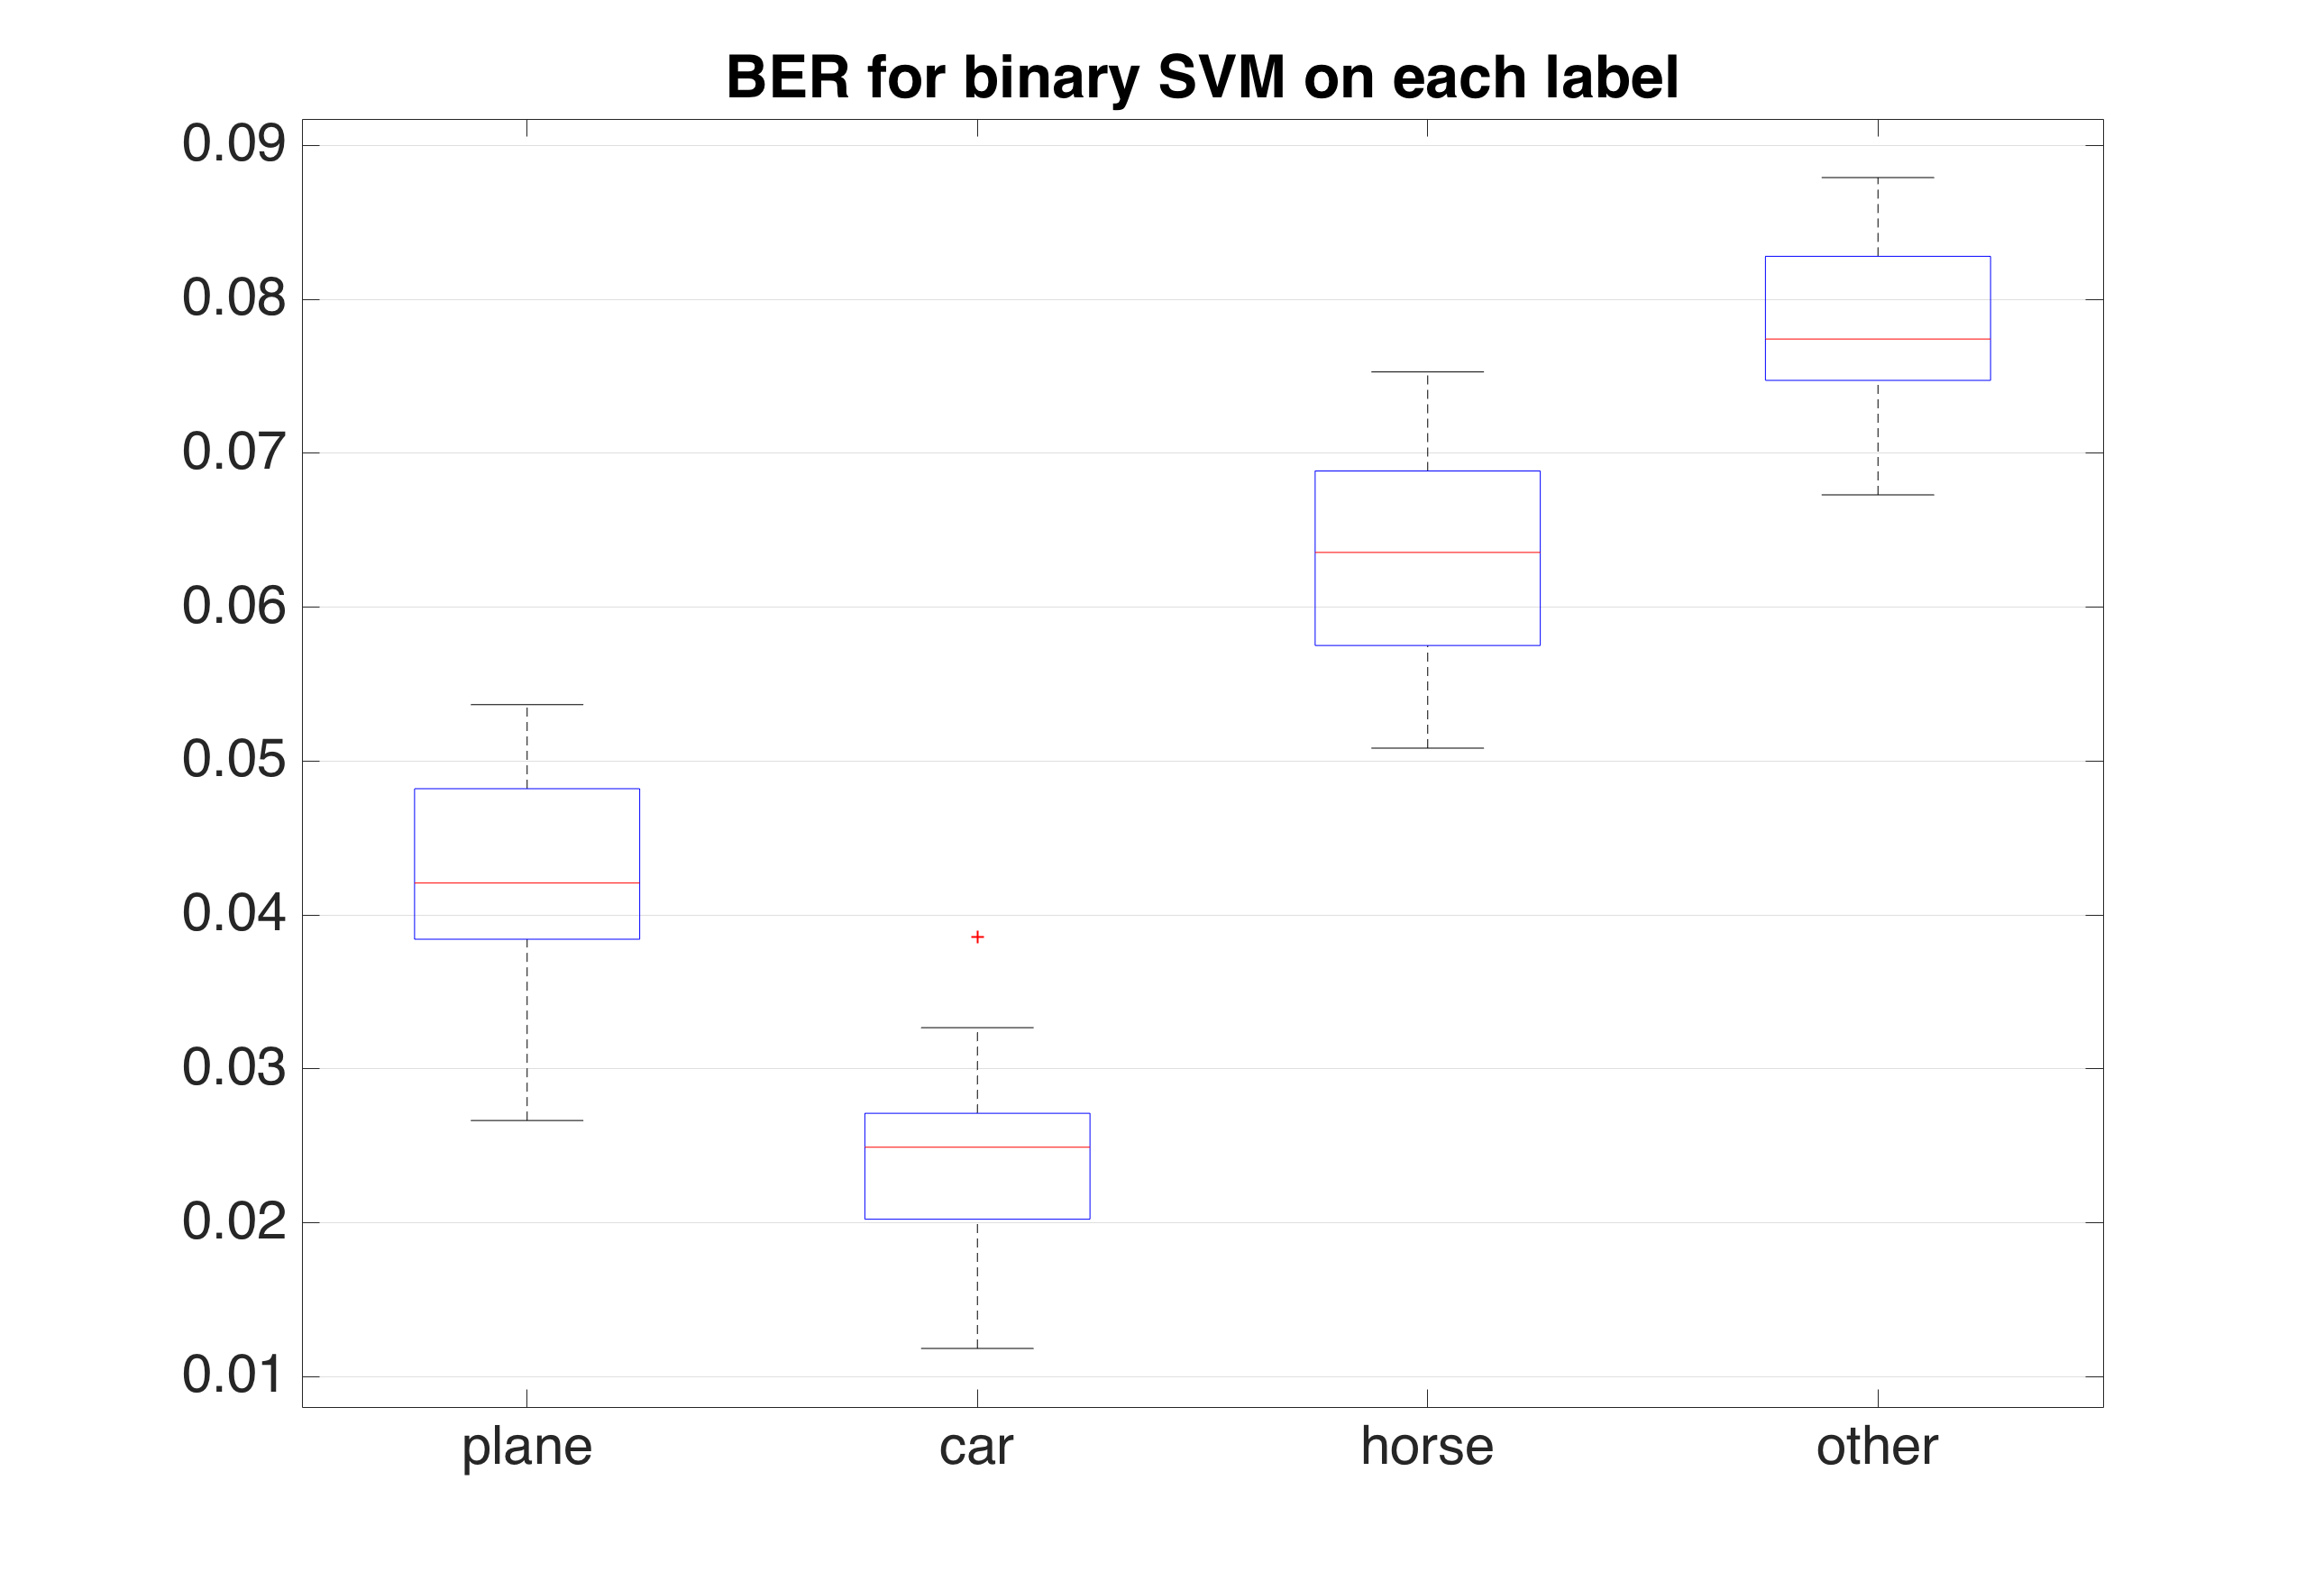
\includegraphics[width=0.7\textwidth]{figures/binaries_svm}
    \caption{Evaluating the RBF SVM methods for the diverse binary classifications}
  	\label{fig:svm-binaries}
\end{figure}

\begin{figure}[h]
	\center
  	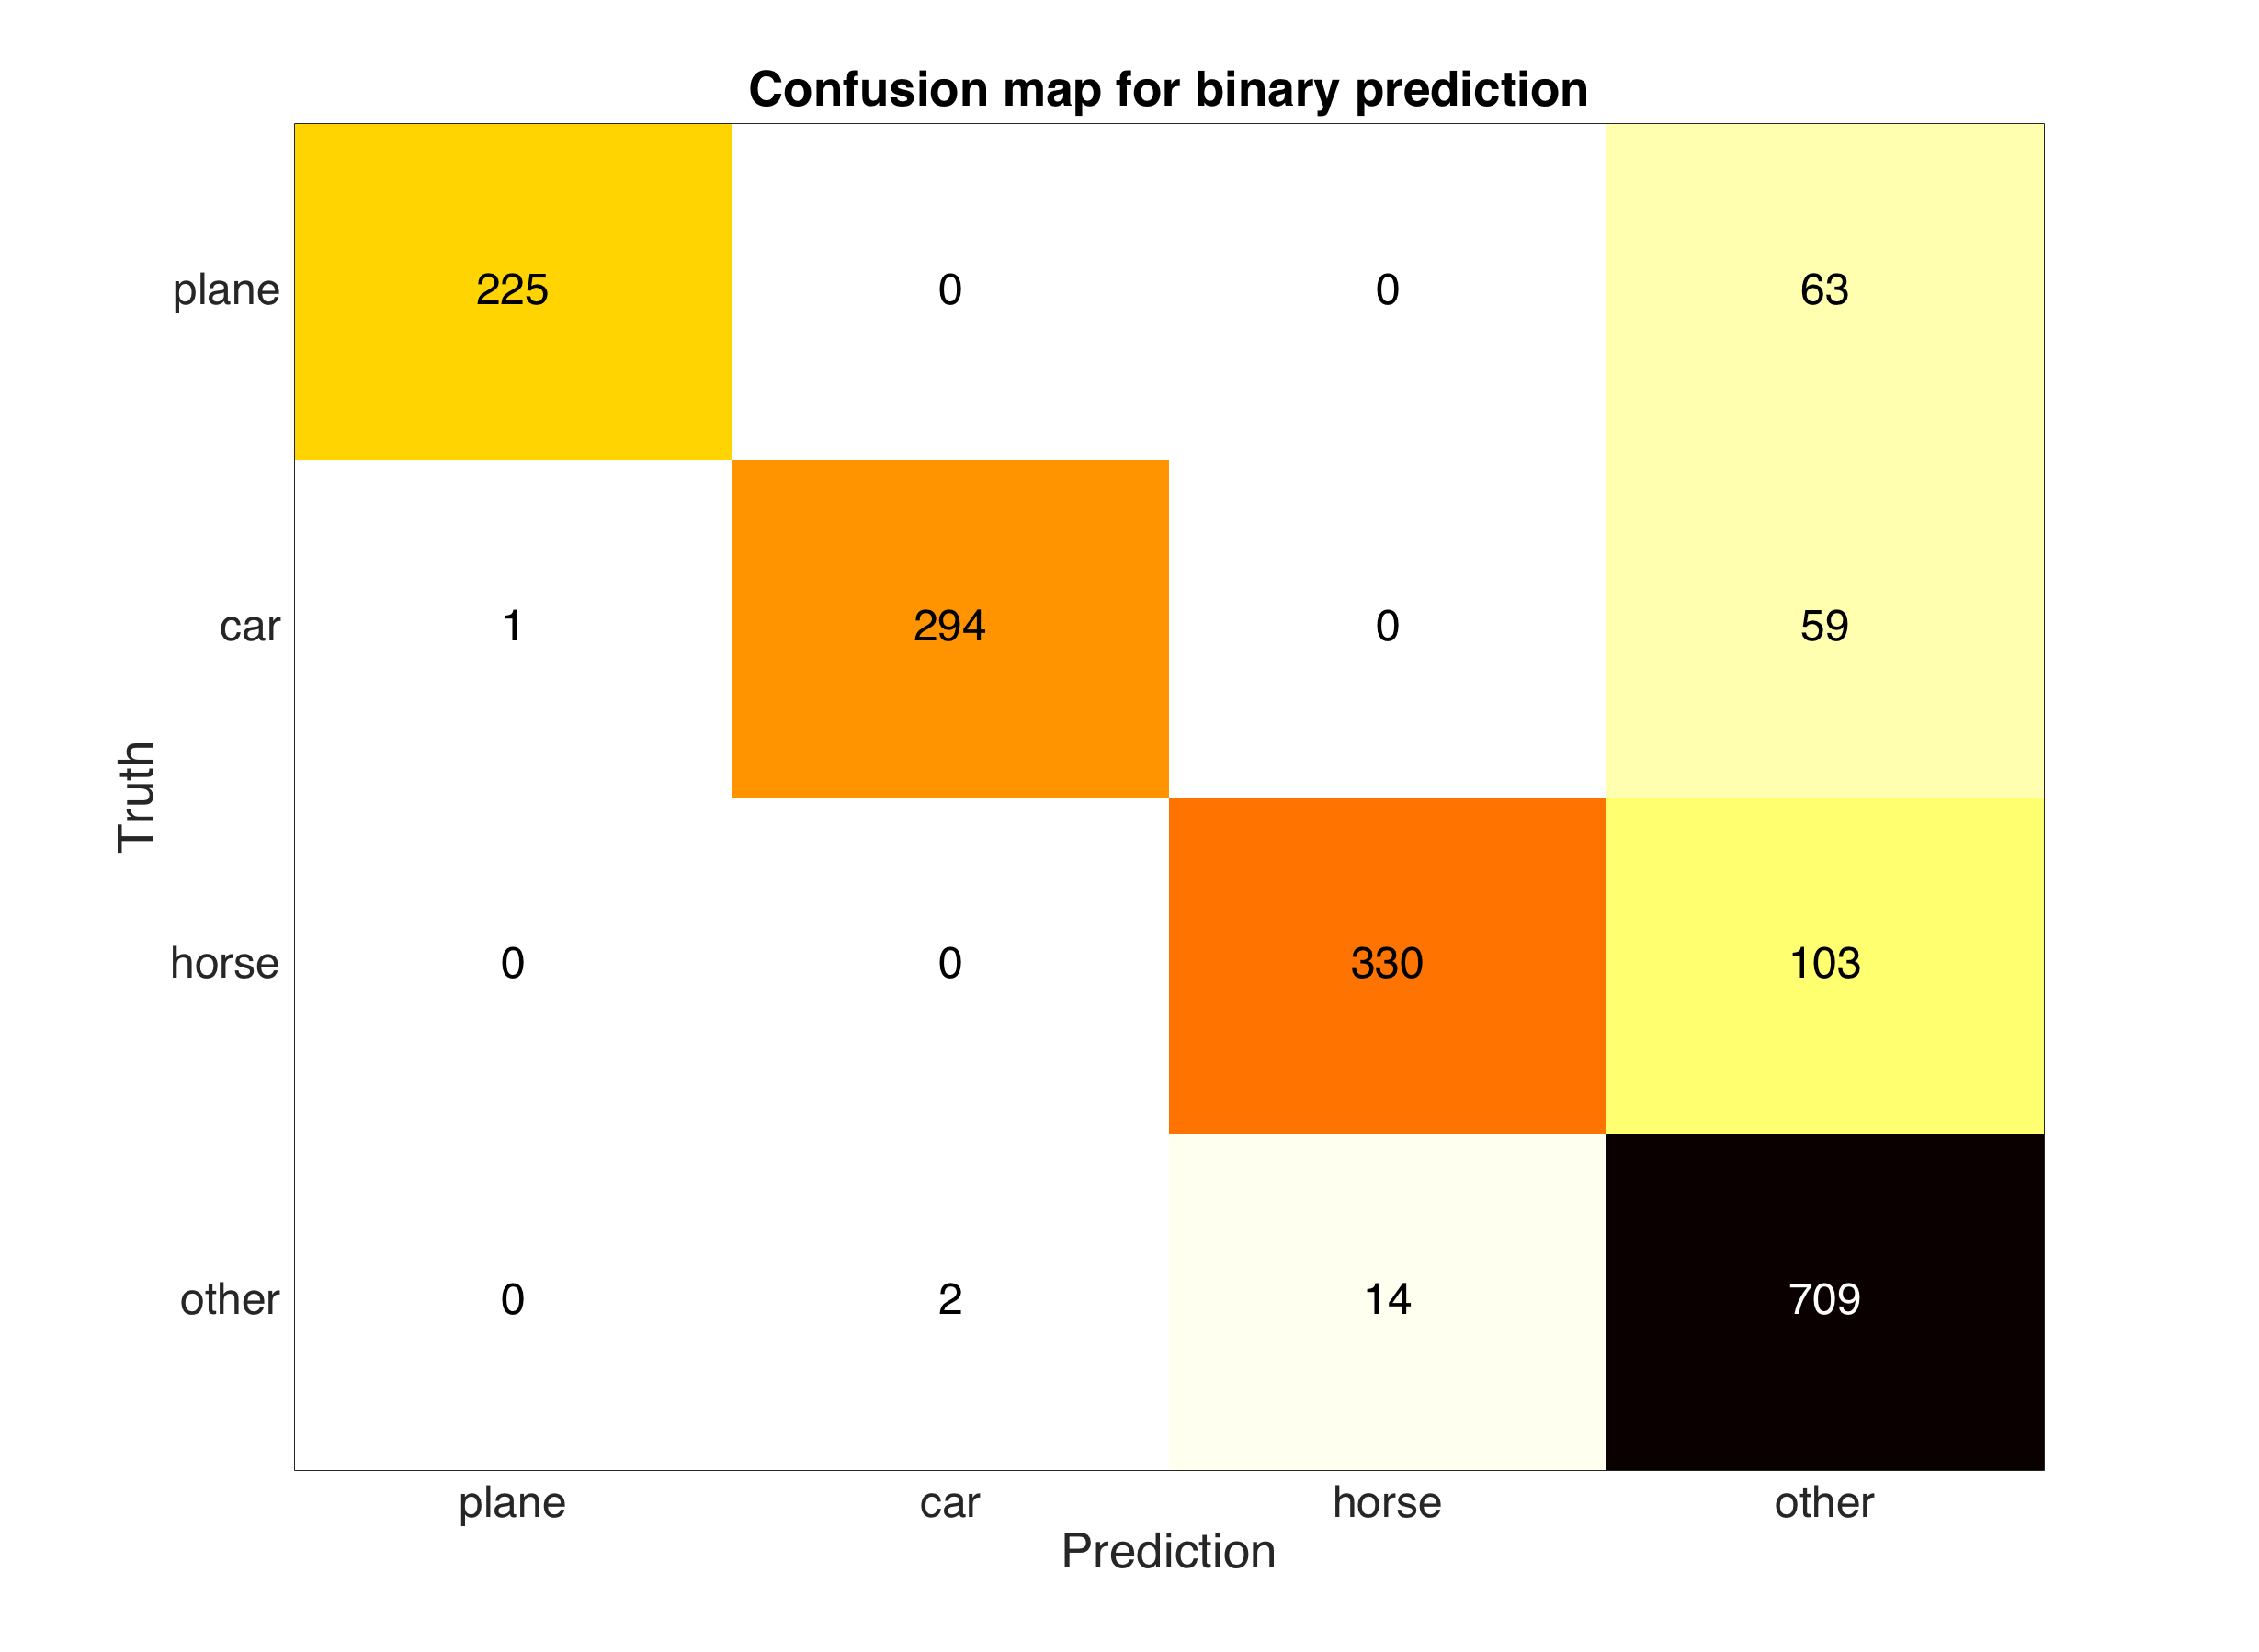
\includegraphics[width=0.7\textwidth]{figures/confusion_map}
    \caption{Confusion matrix for SVM + Manual Tree model}
  	\label{fig:confusion}
\end{figure}

With that in mind, we devised a manual decision tree that, given the prediction scores for labels \textit{car}, \textit{plane} and \textit{horse}, will decide to which of the four classes an image belongs to; i.e. if the score for car is higher than 1, the image is considered to be a car, else if the score for plane is higher that 1, the images falls into the category of planes, and if the confidence to be a horse is more than 1, the image is categorised as one, and otherwise we assume the image is none of those three categories. Using this simple decision tree based on the prior accuracy of each binary classifier, we were able to reach a BER of 7.8\% as depicts in the \textit{SVM + Manual Tree} column of Figure \ref{fig:methods-multiclass}. This strategy does very few errors for images of planes, cars or horses since such as classification implies that a score returned by the SVM classifier is greater than the threshold of $1$, meaning that the classifier is very confident in its decision. Figure \ref{fig:confusion} confirms than most of the false positives are objects from class \textit{plane}, \textit{car} and \textit{horse} classified as \textit{other} with a decision threshold of $1$.
Tuning further this decision boundary and setting it to $0.7$ improved the results to an expected BER of 7.3\% as reported in Figure \ref{fig:methods-multiclass} by the column \textit{SVM + Manual Tree 2}.

Additionally, we compared this approach against the Matlab implementation of SVM for multi-class identification, namely \textit{fitcecoc} with the \textit{'SVM'} learner. Thanks to its auto-tuning ability, we were able to achieve an error of 8.6\% as reported in Figure \ref{fig:methods-multiclass} in the column named \textit{SVM Matlab}. We expect, however, that the error could be slightly improved with this model by manually tuning its parameters instead of fully relying on the heuristic used by Matlab.

Next, we looked into simple one-layer, feed-forward Neural Network as we did for the binary task in Section \ref{sec:binary}, that is we only did a minimal tuning of its inner layer size to avoid overfitting. When applied on the CNN features, we achieved a BER of 9.2\% on average on the validation set. If applied to the HOG features, we were only able to get an average error rate of roughly 30\%.


\begin{figure}[h]
  \center
  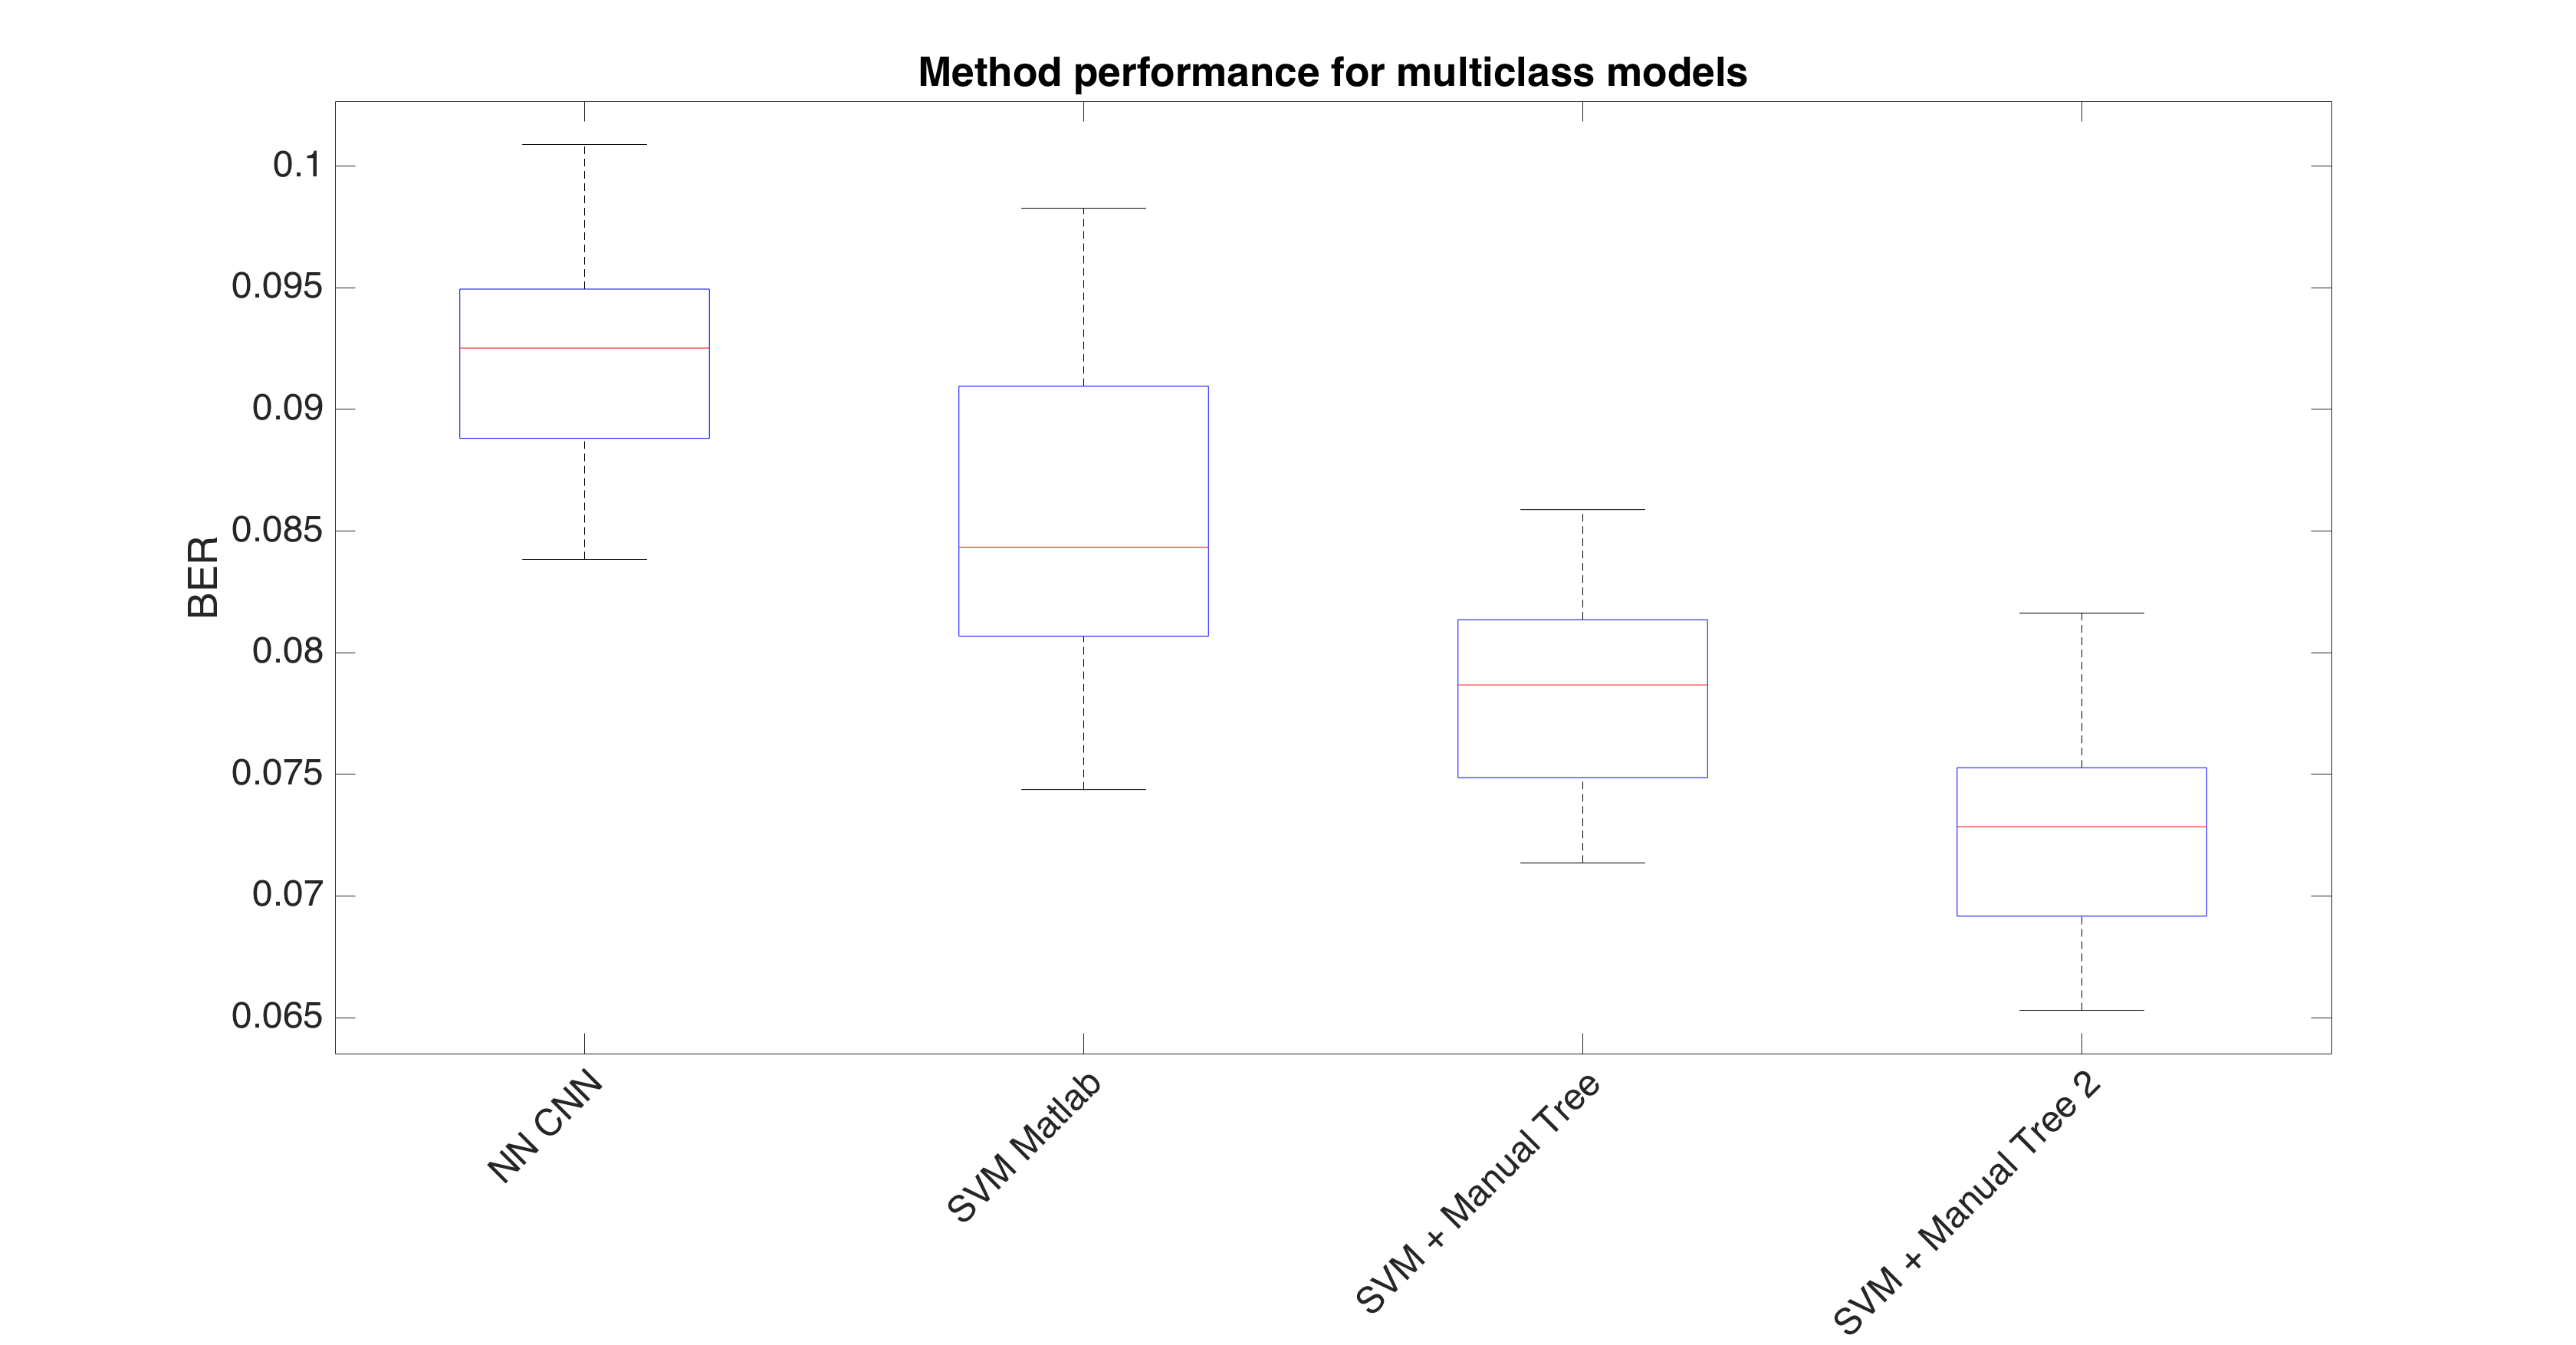
\includegraphics[width=\textwidth]{figures/multiclass_methods}
  \caption{Evaluating the methods for the Multiclass Task}
  \label{fig:methods-multiclass}
\end{figure}


\section{Implementation details}
We implemented the SVM and the PCA algorithm. However, we used the Sequential minimal optimization (SMO) provided during the laboratories for solving the quadratic optimization problem that arises in the SVM algorithm. We also used the Matlab functions such as \textit{svmtrain} for their many options and flexibility in tuning the hyper-parameters.

\section{Results}

To summarise our results, we achieved for the Binary Task an expected BER of $8.18$\% when using the CNN features to train a SVM model that rely on a RBF kernel and a $7.3$\% expected BER for the Multi-class predictions with three binary SVM classifier based on the RBF kernel and a decision tree.

\section{Conclusion}

Given a labelled dataset of images, several methods were evaluated against baselines in their ability to produce good models with low variances. More sophisticated methods proved useful under some conditions such as reducing the dimensionality of the samples and choosing an appropriate error metric for the evaluation.

We encountered many practical aspects of advanced Machine Learning methods such as finding the appropriate range and sweet spots for each of our parameters for best performance while avoiding the overfitting problem.


\subsubsection*{References}
[\textit{HOG}] Dalal, Navneet and Triggs, Bill "Histograms of oriented gradients for human detection" International Conference on Computer Vision \& Pattern Recognition (CVPR ’05), Jun 2005, San Diego, United States. IEEE Computer Society, 1, pp.886–893, 2005.

[\textit{OverFeat}] Sermanet, Pierre, et al. "OverFeat: Integrated recognition, localization and detection using convolutional networks." arXiv preprint arXiv:1312.6229 (2013).

[\textit{Bishop}] Bishop, Christopher "Pattern Recognition and Machine Learning", Springer (2006).

[\textit{PMT}] Piotr Doll\'ar, Piotr's Computer Vision Matlab Toolbox, \url{http://vision.ucsd.edu/~pdollar/toolbox/doc/index.html}

[\textit{DLT}] Palm, Rasmus Berg "Prediction as a candidate for learning deep hierarchical models of data", 2012.

\end{document}

